\documentclass[border=10pt]{standalone}

\usepackage{tikz}
\usepackage{tikzsymbols}
\usetikzlibrary{calc,patterns,shapes.geometric}

\def\centerarc[#1](#2)(#3:#4:#5){\draw[#1] ($(#2)+({#5*cos(#3)},{#5*sin(#3)})$) arc (#3:#4:#5);}

\begin{document}
	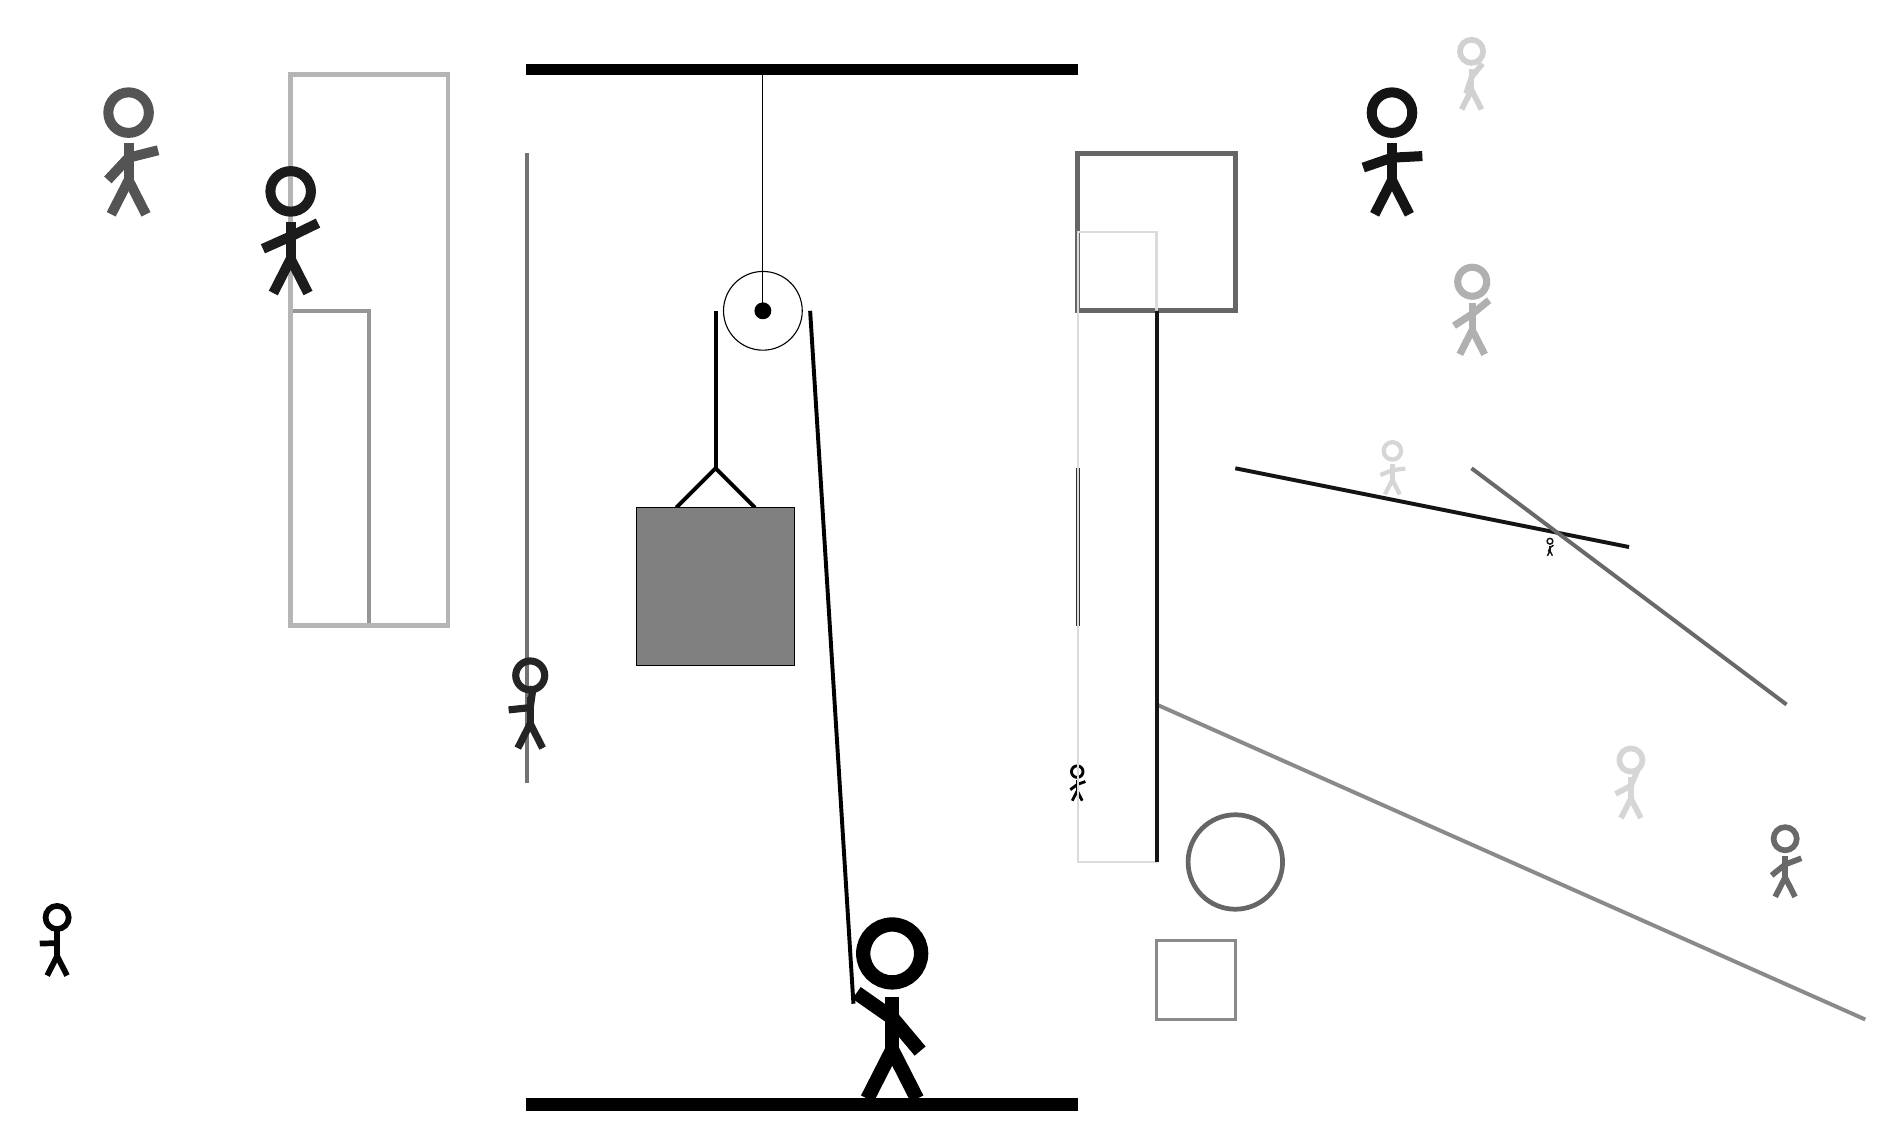
\begin{tikzpicture}
		%%%%% START %%%%%
		
		\draw[fill=black] (-2, 10) rectangle (5, 10.125);
		
		\draw (1, 7) circle (0.5);
		\draw[fill=black] (1, 7) circle (0.1);
		\draw (1, 10) -- (1, 7);
		
		\draw[line width=0.5mm] (-0.1, 4.5) -- (0.4, 5.0) -- (0.9, 4.5);
		\draw[fill=black!50] (-0.6, 4.5) rectangle (1.4, 2.5);
		
		\draw[line width=0.5mm] (0.4, 7) -- (0.4, 5.0);
		\centerarc[line width=0.5mm](1, 7)(0:180:0.6);
		\draw[line width=0.5mm](1.6, 7) -- (2.15, -1.8);
		
		\node at (2.6, -1.9) {\Strichmaxerl[10][-35][-50]};
		
		\draw[line width=0.5mm, color=black!92](7, 5) -- (12, 4);
		
		\draw[line width=0.5mm, color=black!55](-2, 1) -- (-2, 9);
		\node[line width=0.4mm, color=black!99] at (5, 1) {\Strichmaxerl[2][37][20]};
		\draw[line width=0.5mm, color=black!46](6, 2) -- (15, -2);
		\draw[line width=0.5mm, color=black!59](10, 5) -- (14, 2);
		
		\draw [line width=0.4mm, color=black!84](10, 1) circle (0.0);
		\node[line width=0.7mm, color=black!31] at (10, 7) {\Strichmaxerl[5][33][39]};
		\node[line width=0.3mm, color=black!98] at (-8, -1) {\Strichmaxerl[4][1][90]};
		\draw[line width=0.6mm, color=black!60] (5, 7) rectangle (7, 9);
		
		\draw[line width=0.4mm, color=black!46] (6, -2) rectangle (7, -1);
		\draw[line width=0.5mm, color=black!41] (-4, 7) rectangle (-5, 3);
		
		\draw [line width=0.6mm, color=black!60](7, 0) circle (0.6);
		\node[line width=0.7mm, color=black!67] at (-7, 9) {\Strichmaxerl[7][47][14]};
		
		\node[line width=0.6mm, color=black!18] at (10, 10) {\Strichmaxerl[4][72][51]};
		\draw[line width=0.6mm, color=black!29] (-3, 10) rectangle (-5, 3);
		\node[line width=0.5mm, color=black!59] at (14, 0) {\Strichmaxerl[4][39][21]};
		
		\node[line width=0.7mm, color=black!16] at (12, 1) {\Strichmaxerl[4][28][67]};
		\node[line width=0.4mm, color=black!92] at (9, 9) {\Strichmaxerl[7][19][3]};
		\node[line width=0.2mm, color=black!89] at (-5, 8) {\Strichmaxerl[7][24][26]};
		\node[line width=0.5mm, color=black!92] at (11, 4) {\Strichmaxerl[1][69][35]};
		\node[line width=0.6mm, color=black!16] at (9, 5) {\Strichmaxerl[3][22][7]};
		
		\draw[line width=0.5mm, color=black!82](5, 3) -- (5, 5);
		
		\draw[line width=0.3mm, color=black!14] (5, 8) rectangle (6, 0);
		\draw[line width=0.6mm, color=black!29] (-3, 9) rectangle (-3, 10);
		\node[line width=0.6mm, color=black!86] at (-2, 2) {\Strichmaxerl[5][6][82]};
		\draw[line width=0.5mm, color=black!92] (6, 0) rectangle (6, 7);
		
		
		\draw[fill=black] (-2, -3) rectangle (5, -3.15);
		
		%%%%% END %%%%%
	\end{tikzpicture}
\end{document}